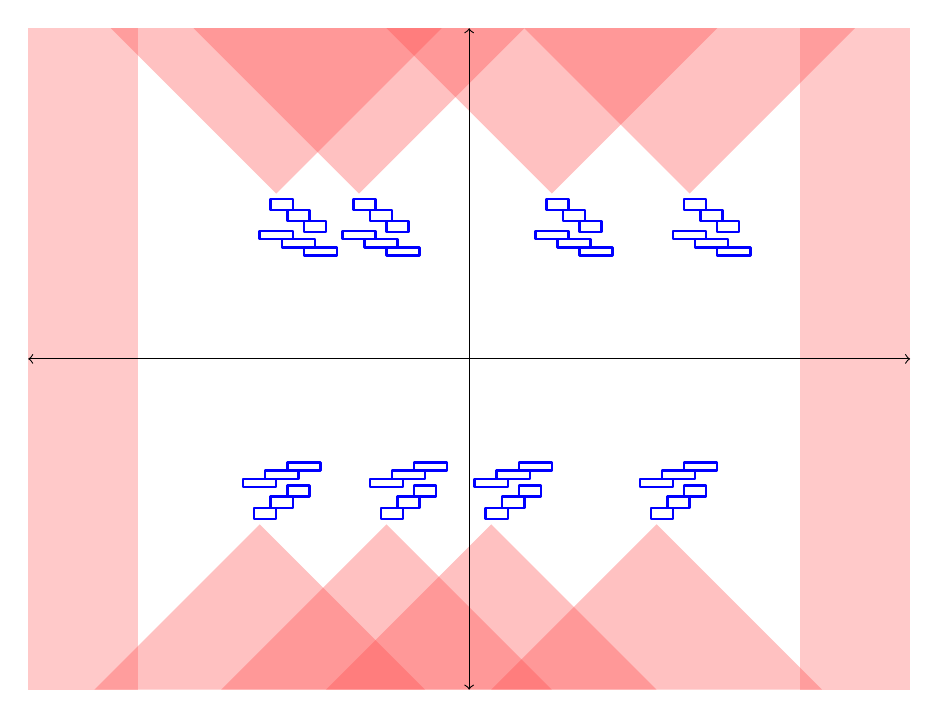
\begin{tikzpicture}[x=0.7cm,y=0.7cm,line cap=round,line join=round]

% convenient parameters
\def\m{3} % number of rectangles per layer
\colorlet{shadeR}{red!70}

% background guide (viewport)
\path (-8,-6) rectangle (8,6);

% red vertical slabs: closest vertical lines with red points (order 1/p away)
\fill[shadeR,opacity=0.30] (-8,-6) rectangle (-6,6);
\fill[shadeR,opacity=0.30] ( 6,-6) rectangle ( 8,6);

% downward cones from the top boundary
\foreach \k in {-3.5,-2,1.5,4}{
  \fill[shadeR,opacity=0.35] (\k-3,6) -- (\k,3) -- (\k+3,6) -- cycle;

  % first two blue layers (top half, mirrored)
  \foreach \i in {1,...,\m}{
    % layer 1
    \draw[blue,line width=0.9pt]
      ({(\i-1)*0.4-\i*0.1+\k}, -\i*0.2 + 3 + 0.1) rectangle
      ({\i*0.4 - \i*0.1 + \k}, -\i*0.2 + 3 - 0.1);
    % layer 2
    \draw[blue,line width=0.9pt]
      ({(\i-1)*0.6-\i*0.2+\k-0.1}, -\m*0.2 - \i*0.15 + 3 + 0.075) rectangle
      ({\i*0.6 - \i*0.2 + \k-0.1}, -\m*0.2 - \i*0.15 + 3 - 0.075);
  }
}

% upward cones from the bottom boundary
\foreach \k in {-3.8,-1.5,0.4,3.4}{
  \fill[shadeR,opacity=0.35] (\k-3,-6) -- (\k,-3) -- (\k+3,-6) -- cycle;

  % first two blue layers (bottom half)
  \foreach \i in {1,...,\m}{
    % layer 1
    \draw[blue,line width=0.9pt]
      ({(\i-1)*0.4-\i*0.1+\k}, \i*0.2 - 3 - 0.1) rectangle
      ({\i*0.4 - \i*0.1 + \k}, \i*0.2 - 3 + 0.1);
    % layer 2
    \draw[blue,line width=0.9pt]
      ({(\i-1)*0.6-\i*0.2+\k-0.1}, \m*0.2 + \i*0.15 - 3 - 0.075) rectangle
      ({\i*0.6 - \i*0.2 + \k-0.1}, \m*0.2 + \i*0.15 - 3 + 0.075);
  }
}

% axes drawn on top
\draw[black,<->] (-8,0) -- (8,0);
\draw[black,<->] (0,-6) -- (0,6);

\end{tikzpicture}